% !TEX root = /Users/royc/Google_Drive/Thesis/RoyC_Umass_Thesis.tex
\chapter{SeqZip - Development and Applications} 
\label{SeqZipMethod} 
\lhead{Chapter 4. \emph{SeqZip - Development and Applications}} 
%----------------------------------------------------------------------------------------
\section{Overview}
  \label{SeqZipMethod:sec:SeqZip Overview}

  Development of SeqZip began with an attempt to circumvent an obvious shortcoming in second generation HTS---short read lengths. Until second generation HTS (i.e. reads <100nt on either the Illumina or SOLiD platforms), most sequencing was done using cloned fragments, stored in a bacteria, and analyzed using dideoxy ``Sanger Sequencing'' (see \ref{Intro:subsec:DNA Sequencing History}). Indeed, this is how most \hyperref[hd:abrevs]{EST}s where analyzed. An extremely powerful feature of these ESTs is that as they represented the sequence of a single original molecule of RNA. Connectivity between sequences that were far apart (>1,000 nt) in the original sequence was maintained. It is this very feature, the continuity of sequence, that allowed whole genome shotgun sequencing to be used, and ESTs to be assembled into complete genomes, despite sometimes lengthly, repetitive, stretches of DNA (see section \ref{Intro:subsec:DNA Sequencing History}). Once research transitioned over to heavy use of the second generation HTS, all of that connectivity was lost, and all the inherent information with it.

  Second generation HTS can be supplemented with other technologies. This has been demonstrated perhaps most successfully with long-read assisted genome assembly \citep{Koren2012a}. Why not supplement the disconnected nature of short reads with another technology? To that end, Phillip D. Zamore proposed an RNA-templated DNA-DNA ligation approach as drawn in Figure \ref{SeqZipMethod:fig:Original SeqZip Diagram} (see US Patent application \href{http://1.usa.gov/PTG9BB}{12/906,678}). Using this approach, two or more distant sequences of RNA are investigated using short DNA oligonucleotides that force the intervening sequences to loop out. Incorporation of the hybridized DNA via ligation with those of DNAs adjacently hybridized generates a positive readout of sequence presence.

  \begin{figure} % Original SeqZip Diagram
    \centering 
    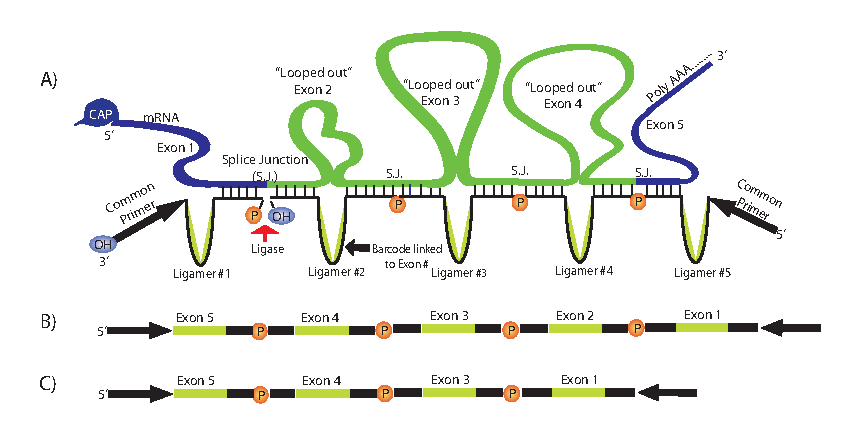
\includegraphics{Figures/SeqZipMethod/OriginalSeqZipDiagram.eps}
    \caption[Original SeqZip Diagram]
    {
      Original SeqZip Diagram\\[0.25cm]
      The original concept diagram of the SeqZip methodology. (A) Specific DNA oligos target an mRNA and loop out the RNA sequence. Ligases is added to join the DNA oligos together; (B) \& (C) Two different possibilities of ligation products templated from the RNA in (A), where Exon 2 is an cassette exon.
    	}
    \label{SeqZipMethod:fig:Original SeqZip Diagram}
  	\end{figure}

  Along with Patent \href{http://1.usa.gov/PTG9BB}{12/906,678}, Chapter \ref{SeqZipPaper} presents much of the early and important developmental work demonstrating reduction to practice of this method (termed ``SeqZip"), and its application to investigating connectivity of sequence content in the biologically-interesting genes \fn{} and \dscam{}. 

  Presented in this Chapter are experiments demonstrating SeqZip application to the following questions and issues:

  \begin{itemize} % Itemized list of sections
    \singlespacing
    \item Section \ref{SeqZipMethod:sec:Multiplex Gene Study}: 
      Simultaneous investigation of 10 genes ("Multiplex") for coordinated alternative splicing.
    \item Section \ref{SeqZipMethod:sec:RNA Integrity via SeqZip}: 
      Investigate of RNA integrity using SeqZip.
    \item Section \ref{SeqZipMethod:sec:piRNA precursor by SeqZip}: 
      Demonstrating the presence of long, continuous piRNA precusors by SeqZip
	  \end{itemize}

  The three sections add to the data discussed in Chapter \ref{SeqZipPaper} in some important ways. Section \ref{SeqZipMethod:sec:Multiplex Gene Study} demonstrates that SeqZip can not only be used to investigate an extremely complex alternatively spliced gene (\dscam{}) in a comprehensive manner, but can also be applied to looking at multiple genes at once. Section \ref{SeqZipMethod:sec:RNA Integrity via SeqZip} exploits a subtle feature of the method---that the RNA must be intact in order to produce a ligation product. This can be used to report on a fraction of intact RNA and deduce meaningful information such as the amount of intact RNA virus, or the existence of as-yet unobserved mega transcripts, like mammalian piRNA precursors (section \ref{SeqZipMethod:sec:Demonstrating continuous precursor TX by SeqZip}).

\section{Multiplex SeqZip Application}
  \label{SeqZipMethod:sec:Multiplex Gene Study}

  Is the coordination discussed in section \ref{Intro:subsec:Coordination in splicing} a general phenomenon? One of the major goals of developing SeqZip was to investigate potential coordination genome-wide. By genome-wide, what we really mean is to analyze many (or all) of the RNA transcripts in a tissue for evidence of coordinated splicing decisions. When development of the method reached the point that it could be applied to a multiplex study, I did not posses the bioinformatic skills necessary to (1) identify target transcripts, exons, and sequences to investigate for potential connectivity and (2) design ligamers in an automated and high-throughput fashion. Both of these points are discussed later (see \ref{SeqZipMethod:sec:Demonstrating continuous precursor TX by SeqZip} and \ref{Disc}).

  In order to make some progress on applying the technique to multiple genes at once, I used data presented by \citet{Fagnani2007}. This paper identified genes displaying tissue-specific splicing patterns, focusing on those with CNS-specific patterns. One section focused on ``Coordination between alternative splicing events belonging to the same genes,'' and seemed to be the exact type of genes we were interested in applying SeqZip too. Five hundred of the 3,044 genes investigated by their microarrays contained 2\textendash 5 alternative exons. \citet{Fagnani2007} contained an additional data file listing all pair-wise combinations of alternative exons in the same gene (with that gene having significant expression in >20 different tissues) along with the standard and partial spearman correlations. 

  It is important to note that the genes above also contain alternative first exons, a prominent type of alternative splicing (Figure \ref{Intro:fig:asEventsBarChart}). Indeed, from microarrays studies, it has been estimated that approximately 16\%\textendash 23\% of all alternative splicing events involve alternative first and last exons \citep{Bingham2008}. It is known that, through alternative use of first and last exons, cells can fine-tune a transcript's untranslated region (UTR) and control many aspects of mRNA regulation including nuclear export, localization, expression, and stability \citep{Hughes2006}.

  Using the \citet{Fagnani2007} data, I filtered exon pairs to those with a distance >350 nt between exons in the final pre-mRNA. I also visualized their transcript architecture, and EST evidence using NCBI's AceView tool \citep{Thierry-Mieg2006}. For example, the exons with strong correlation of expression in \textit{Chl1} are in the beginning (second exon) and end (fourth from last exon, accession BC060216) with plenty of supporting evidence for these exons being expressed and skipped. After combing through \citep{Fagnani2007} data, I assembled a list of 11 genes (Table \ref{table: BigSpanGenes}) to investigate for coordinated splicing.

  \begin{table} % Big Span Genes in mice from Fagnani 2007
    \caption[Mouse genes with large sequence between suggested coordinated cassette exons]
      {
        A list of 11 genes investigated in section \ref{SeqZipMethod:sec:Multiplex Gene Study}. Coordination between exons first suggested by \citep{Fagnani2007}.
        }
    \label{table: BigSpanGenes}
    \begin{table}[h]
\begin{tabular}{|l|r|r|r|r|}
\hline
\textbf{Gene name} & \textbf{nt of mRNA between exons} & \textbf{possible isoforms} & \textbf{Exon 1} & \textbf{Exon 2} \\ \hline
Chl1               & 4665                              & 18                         & 2               & 24              \\ \hline
Mdm1               & 1846                              & 4                          & EDA             & IIICS           \\ \hline
PTPRF-Y            & 1633                              & 4                          & 2               & 13              \\ \hline
Cacna1c            & 1403                              & 4                          & 15              & 21/22           \\ \hline
PTPRF-X            & 936                               & 4                          & 9/10            & 21              \\ \hline
FN1                & 813                               & 8                          & 13/14           & 21/22           \\ \hline
Apbb1              & 802                               & 260                        & 1/2b            & 2/3e            \\ \hline
Agrn               & 736                               & 8                          & 33/34c          & 33/34a          \\ \hline
Exoc7              & 513                               & 4                          & 7               & 13              \\ \hline
Prom1              & 512                               & 4                          & 7               & 9               \\ \hline
Lphn2              & 396                               & 32                         & 19              & 24/25a          \\ \hline
\end{tabular}
  \caption[Genes with big spans in between]{\hl{caption}}
  \label{table: BigSpanGenes}
\end{table}

    \end{table}

  I hand-designed ligamers for each of these genes. Ligamers were ordered from IDT in a 96-well plate format, pooled according to gene, and used to develop a multiplex approach to applying SeqZip. I used total RNA from mouse brains as the input material.

  \begin{figure} % 11 Gene Set Schematic
    \centering 
    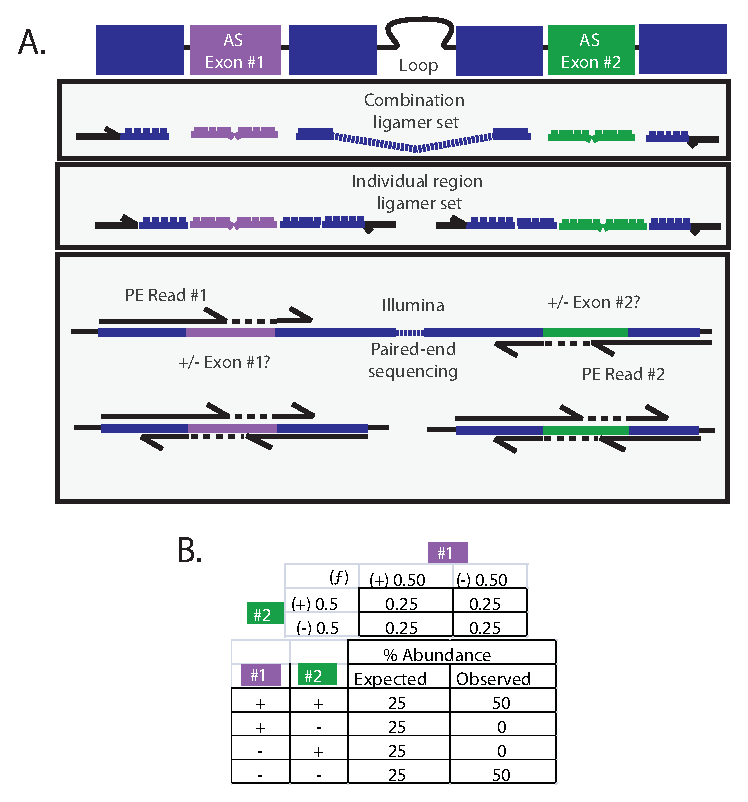
\includegraphics{Figures/SeqZipMethod/10GeneSetSchematic.eps}
    \caption[10 Gene Set study schematic]
    {
      11 Gene Set study schematic\\[0.25cm]
      A) Two pools of ligamers, ``Combination'' and ``Individual,'' were used to investigate splicing of cassette exons individually or while maintaining connectivity. Ligation products were sequenced on the Illumina platform using a paired-end approach. B) A hypothetical example of showing how individual splicing rates can confound true isoform identity when observing regions independently.
	    }
    \label{SeqZipMethod:fig:Multiplex Study Design}
  	\end{figure}

  After attempts to perform SeqZip on all 11 genes in one ligation failed, I reverted back to \textit{per-gene} ligation reactions in order to trouble shoot and optimize the assay. Once I had obtained ligation products from per-gene ligation reactions for both the individual and combination ligamers pools, I pooled all the ligation products and amplified them. Amplified products were sent for paired-end 100 sequencing on the Illumina GEIIx platform. 

  After considerable delay and optimization from the Umass Sequencing Core due to low library sequence diversity, the analyzed data demonstrated little alternative splicing in the genes examined. Put another way---most of the transcripts observed via SeqZip were uniform in exon inclusion and showed little variation for cassette exon inclusion (Figure \ref{SeqZipMethod:fig:Apbb1 Results}). These results forced us to rethink applying SeqZip to multiple genes or complex alternative splicing (i.e. \dscam{}). For most genes, there was too few reads aligning to combination products, arguing for more careful mixing of the more efficient individual products with lower-efficiency combination products prior to sequencing. For a discussion of different type of multiplex study, see section \ref{Disc:subsec: Ideal SeqZip exp. to look for Coordination}.

  \begin{figure} % Appb1 Multplex example
    \centering 
    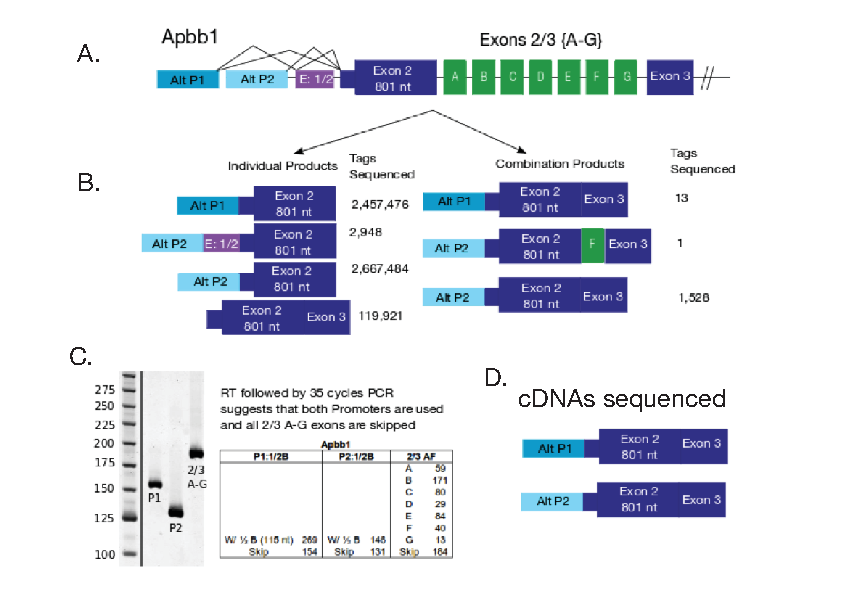
\includegraphics{Figures/SeqZipMethod/Apbb1.eps}
    \caption[Measuring \textit{Apbb1} via SeqZip in multiplex study]
    {
      Measuring \textit{Apbb1} via SeqZip in multiplex study\\[0.25cm]
      A) Region of \textit{Apbb1} investigated. Two alternative promoters, a 5\textprime~cassette exon (``E:1/2'') and a 3\textprime~group of cassette exons (``Exon 2/3 \{A--G\}''). B) Number of sequencing reads mapping to individual \textit{Apbb1} ligation products (left) and combination (right). C) RT-PCR of total RNA taken from a mouse brain looking for cassette exon usage at each position shown in (A). Also shown in the size in nt of the expected bands. D) Schematic of cDNAs cloned and sequencing from mouse brain total RNA.
      }
    \label{SeqZipMethod:fig:Apbb1 Results}
    \end{figure}

\section{RNA Integrity}
  \label{SeqZipMethod:sec:RNA Integrity via SeqZip}

  An exciting use of SeqZip is rapid quantification of RNA integrity. Integrity defined as the faction of molecules that are continuous and unbroken nucleic acid polymers, from the original site of transcript to 3\textprime~processed end. Quantification of integrity has many uses including: (1) quality control of RNA before downstream analysis such as RT or sequencing, and (2) implications of infectivity for viruses that package RNA genomes in virions.

  \subsection{Demonstration of Concept}
    \label{SeqZipMethod:subsec:SeqZip can be used to examine viral genomes}

    In order to demonstrate the feasibility of the SeqZip assay toward performing these type of analysis, I \textit{in vitro} transcribed a 9,800 nt long RNA that I digested using ZnCl$_{2}$ at two different concentrations and times (Figure \ref{SeqZipMethod:fig:Ligation product and RNA integrity}). The RNA was probed using three ligamers, two to the very edges of the RNA and one that looped out the intervening 8,000 nt. The amount of product observed should be directly tied to the abundance of the full length template.

	  \begin{figure} % Degraded RNA measurement by SeqZip
    	\centering 
    	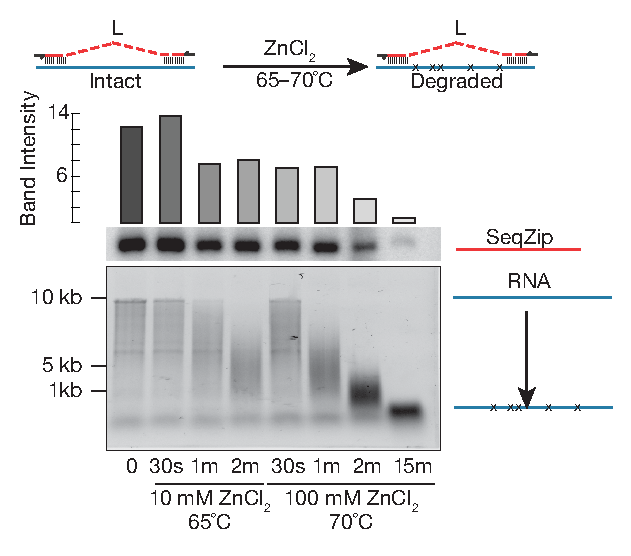
\includegraphics{Figures/SeqZipMethod/DegreadedRNABySeqZip.eps}
    	\caption[Ligation product tied to RNA integrity]
    	{
		    Ligation product tied to RNA integrity\\[0.25cm]
      	Top) Schematic demonstrating SeqZip analysis of transcript integrity. A middle ligamer (L), that hybridizes to the edges of a 8,000 nt section of RNA should only ligate to flanking ligamers when the template RNA is intact. \\
        Middle) Intensity of PCR products amplified using end-labeled primers such that the intensities of all bands can be quantitatively compared (i.e. semi-quantitative PCR). Bottom) A denaturing agarose gel stained with EtBr showing the intactness of the template RNA used in position-matched ligation reactions in the middle panel.
    		}
    	\label{SeqZipMethod:fig:Ligation product and RNA integrity}
  		\end{figure}

    Figure \ref{SeqZipMethod:fig:Ligation product and RNA integrity} shows promising results toward the ability of SeqZip to report on RNA integrity. The apparent intensity of the bands shown in (middle) was tied to the amount of intact RNA seen in (bottom). However, the lane where the RNA was degraded for two minutes with 10 mM ZnCl$_{2}$ compared to 30 seconds with 100 mM ZnCl$_{2}$ were not in good agreement, with clearly less intact RNA in the two minute lane, but just as much ligation product. We hypothesized that this was due to inherent secondary structure in the template we used (a section of the HIV genome, discussed in section \ref{SeqZipMethod:sec:RNA Integrity via SeqZip}). 

    At what concentration of template do ``long'' ligamers generate ligation products from template fragments? Using pools of ligamers targeting fragments and the complete template (the same template used in Figure \ref{SeqZipMethod:fig:Ligation product and RNA integrity}). SeqZip was performed using a 1:1 ratio of RNA fragments. Results (Figure \ref{SeqZipMethod:fig: trans Tx for degradation}) show that SeqZip accurately reports on the presence of fragments, and not full length transcripts at $\le$1 nM template. This is in good agreement with results presented in Chapter \ref{SeqZipPaper}.

  	\begin{figure} % Trans RNA with SeqZip
    	\centering 
    	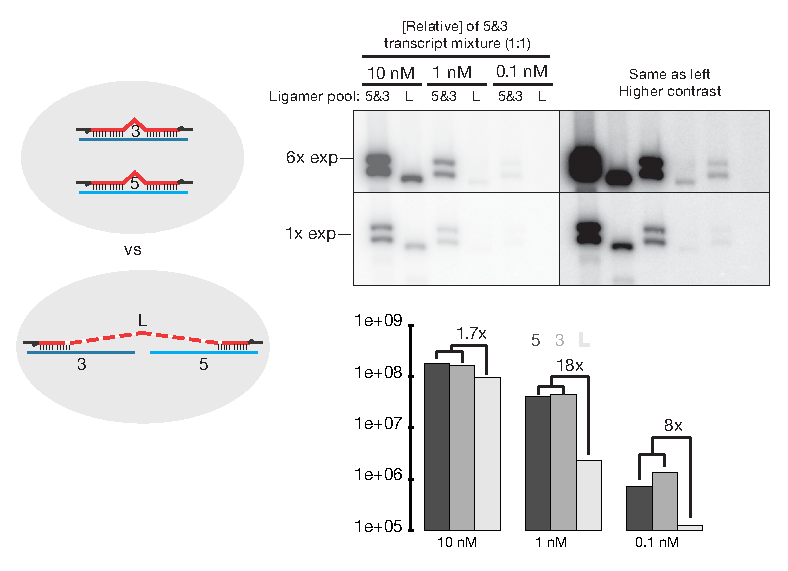
\includegraphics{Figures/SeqZipMethod/TransRNAWithSeqZip.eps}
    	\caption[Trans Transcript investigation]
    	{
	      \textit{Trans}-transcript investigation\\[0.25cm]
  	    Left) Schematic of experimental design: Three pools of ligamers were used. Two (labeled ``3'' and ``5'') hybridize to the 5\textprime~and 3\textprime~sections of a 9,800 nt template RNA. The last, labeled ``L'' connects these two regions via a long longer with target 5\textprime~and 3\textprime~regions of complementarity. (Right;Top) Combinations of the ligamer pools were used with different concentrations of template RNA in the SeqZip assay. Ligation products were amplified with end-labeled PCR primers and amplified using radioactive PCR. Shown are low (left column) and high (right column) versions of two different exposure times (1x on bottom and 6x on top). Right Bottom) Quantification of the bands shown in the gel above, grouped by input template RNA concentration. The fold difference in band intensity between the lowest signal ``5'' or ``3'' ligamer pool and the ``L'' pool is indicated. Y-Axis is the raw band intensity.
		    }
   	 \label{SeqZipMethod:fig: trans Tx for degradation}
	 	 \end{figure}

     These results are encouraging, but bear repeating in order to address the issues of potential secondary structure and repetitive regions inherent to the template RNA used. Put differently---they should be repeated with a traditional mRNA template, instead of a highly-structured and repetitive RNA such as the HIV genome.

  \subsection{HIV Genome Integrity}
    \label{SeqZipMethod:subsec: Why use SeqZip to look at HIV genomes}

    In late 2010--early 2011, a graduate student in the \href{http://profiles.umassmed.edu/profiles/display/133484}{Gottlinger} lab, Anna Kristina Serquiña observed that a cell line expressing ATPase-defective forms of the SF1 helicase UPF1 \citep{Bhattacharya2000} did not infect reporter cell lines the same as control. Previous mass-spec results had reported MOV10 (a SF1 family helicase \citep{Gregersen2014}) was packaged into extracellular viral particles. Anna hypothesized that the decrease in infectivity was due to a problem with RT when the genetic material is introduced into target cells. The results of this study were recently published \citep{Serquina2013}.

    Anna was interested in using SeqZip to quantify intact HIV virus in virus-producing cells and extracellular virions. The first step in applying SeqZip to HIV was to design ligamers.

	\subsection{HIV Ligamer Design}
    \label{SeqZipMethod:subsec: Design of HIV ligamers}

	  Research into the integrity of the HIV RNA genome using SeqZip began with designing a set of ligamers against two different clones. The first, targeting transcripts from the M19921 plasmid (so called ``M'' clone), and the section from the K03455 clone containing nearly identical sequence. We targeted a difference in sequence for one site of ligation (\ref{SeqZipMethod:fig:Hiv tx via SeqZip})A). Three different pools of ligamers were created: a Five(5) ligamer pool, with three ligamers designed to test for the presence of sequence in the first 1,140 nt of the HIV genome, importantly the first site of ligation in the 5 region pool contained a mismatch in the K clone sequence; a three(3) pool, testing the last 1,210 nt of the genome, and a Long (L) ligamer pool, also containing three ligamers, but the middle ligamer of which spans the 5 and 3 regions, looping out 8,633 nt of sequence in the middle of the HIV genome. 

    \textit{In vitro} transcripts were created using both the K and M clones. These transcripts were added to a background of total MEF RNA, and SeqZip was performed. Ligation products were successfully amplified from all ligamer pools when using the M clone transcript and all three ligamer pools. The abundance of these ligation products, as measured by endpoint PCR, seemed to be spike-concentration dependent. Notably, ligation products were not obtained from the K clone using either the 5 or L ligamer pools, likely due to the mismatch between the transcript and the ligamers at the site of ligation. Also of note was the appearance of ligation products from purified endogenous virions of the M clone from all three ligamer pools, and the absence of products from virions purified from plasmids containing a defective protein, Gag, essential for viral packaging. 

	  \begin{figure} % HIV Via SeqZip
  	  \centering 
	    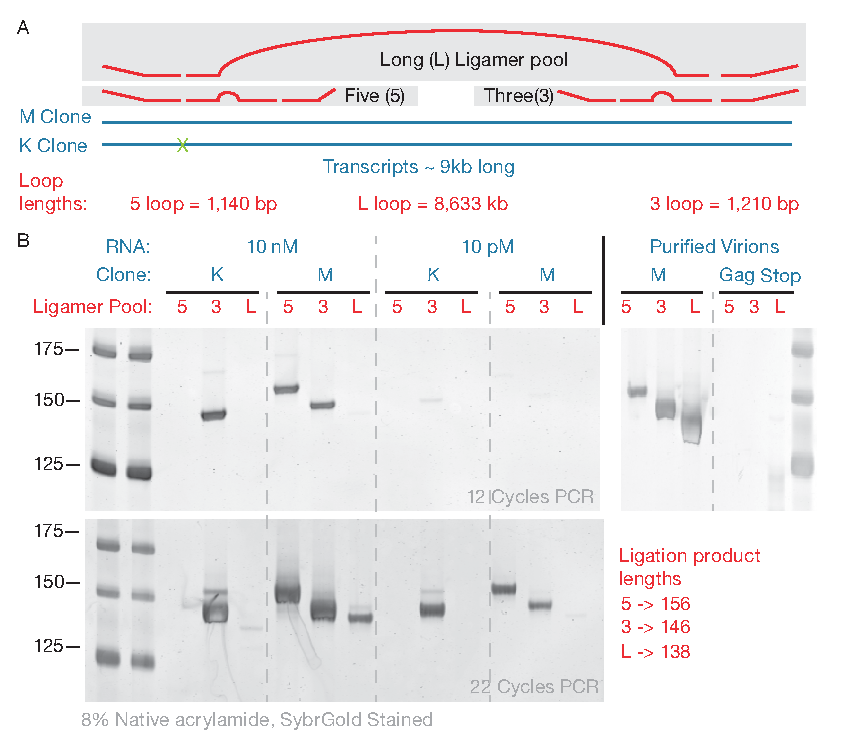
\includegraphics{Figures/SeqZipMethod/HIVviaSeqZip.eps}
    	\caption[SeqZip can examine HIV transcript integrity]
    	{
	      SeqZip can examine HIV transcript integrity\\[0.25cm]
      	A) Schematic demonstrating the experimental design. Three different pools are used to probe for connectivity on the 5\textprime~(Five(5)) and 3\textprime~(Three(3)) ends. Additionally, a Long (L) ligamer is used to check for connectivity between the two ends. We used two different clones of the HIV genome, described in the text and denoted as ``M'' and ``K''. Important here is that the ``K'' contains difference base at a ligation site of the 5 ligamer pool.
        B) A series of end-point PCR gels showing amplified ligation products templated with \textit{in vitro} transcribed RNA at 10 nM or 10 pM of either the K or M clones, or from purified virions of (M clone origin). Show are two different end points of PCR, 12 cycles (top) or 22 cycles (bottom). Also shown is a legend of expected ligation products lengths
    		}
    	\label{SeqZipMethod:fig:Hiv tx via SeqZip}
  		\end{figure}

    The results show (Figure \ref{SeqZipMethod:fig:Hiv tx via SeqZip}) that SeqZip and these three pools of ligamers can be used to profile \textit{in vitro} HIV transcripts and RNA from purified virions. Important features of the figure are: (1) Ligation products are \textit{not} observed for ligation reactions using the K clone template RNA and the Five(5) pool of ligamers, verifying the specificity of the ligamers to the different base of the M clone; and (2) the amount of product from reactions using the L pool of ligamers required more cycles (22 vs 12) in order to be visualized, as would be expected given the physical constraint of hybridizing to two sequences separated by >8,000 nt. 

    Access to purified material and a general push to publish Anna's UPF1 story lead the Gottlinger lab to substantiate the viral genome integrity claims effecting infectivity using a traditional northern blot \citep{Serquina2013}. However, these results are encouraging warrant additional optimization and application of SeqZip to RNA integrity measurements.

\section{piRNA Precursors}
  \label{SeqZipMethod:sec:Demonstrating continuous precursor TX by SeqZip}

  The first genome-wide studies of piRNAs in \flies{} suggested their production from a long, single-stranded RNA, as discussed in section \ref{Intro:sec:Nucleic Acid Polymers} \citep{Brennecke2007,Gunawardane2007}. Yet, demonstration of precursor transcripts existing as continuous, long, RNA molecules had, as of 2010, yet to be demonstrated. If it could be shown through experimentation that precursors existed as long RNAs, it would provide valuable clues as to their biogenesis, included how such a long RNA is packaged and transported around the cell. With these goals in mind, the following section describes efforts to demonstrating the continuity of precursor transcripts using SeqZip.

  \subsection{Mammalian piRNA Precursor Loci}
    \label{SeqZipMethod:subsec:Mammalian Loci of precursor Tx}

    Chapter \ref{MolCel} discuses 214 genomic loci that account for >95\% of all pachytene piRNAs. Many of these loci are intergenic. That is they reside many thousands of base pairs away from another protein-coding gene. Yet many of these loci \textit{are} traditional protein coding genes themselves, making investigation into their eventual biogenesis to mature piRNAs more complicated. Finally, some loci are generated from what appear to be bidirectional promoters. Figure \ref{SeqZipMethod:fig:precursor Loci Locations} shows the location of each of these types of precursor loci on each of the 19 autosomal chromosomes of the mouse. There were no loci identified on the X and Y chromosomes, likely due to transcription silencing during gametogenesis. 

    \begin{figure} % Precursor Transcript Summary
      \centering 
      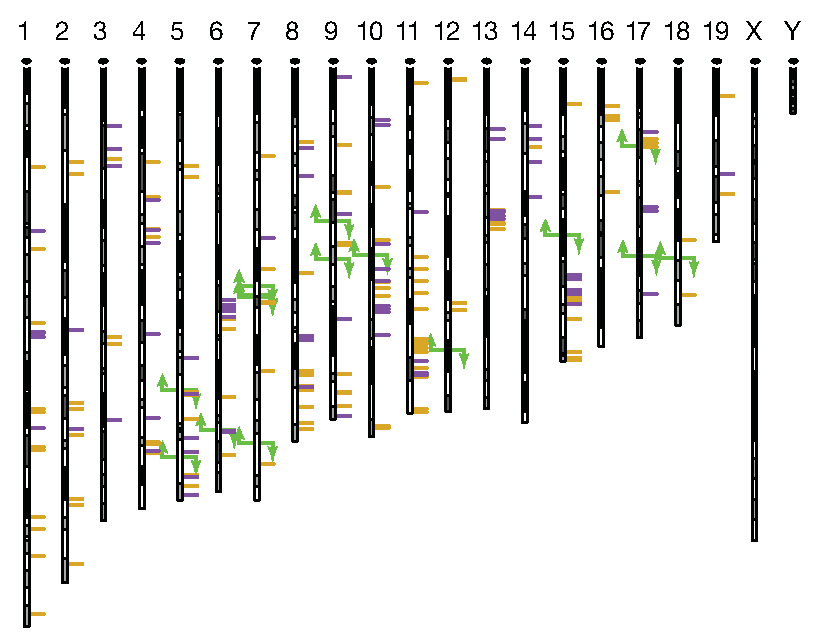
\includegraphics{Figures/SeqZipMethod/PrecursorLocations.eps}
      \caption[Pachytene piRNA precursor locations in mice]
      {
        piRNA precursor locations in mice\\[0.25cm]
        Shown are the 19 autosomal and 2 allosomal mouse chromosomes. They are banded according to ideogram staining and oriented with the centromere (dark black circle) on the top. Yellow bars indicate the location of classified ``pre-pachytene'' loci, which are mostly coincident with previously annotated mRNAs. Purple bars indicate pachytene loci, and are usually far from any other annotated transcript. Finally green arrows, pointing in opposite directions, represent those pachytene loci that are divergently transcribed from a single promoter.
     	 }
      \label{SeqZipMethod:fig:precursor Loci Locations}
      \end{figure}

    The bidirectionally-transcribed sub-type of the pachytene loci are extremely interesting and useful. A motif search of the small sequence between the annotated 5\textprime~TSSs of these transcripts allowed for identification of A-MYB as the transcription factor that drove loci transcription (see section \ref{MolCel:subsec:A-Myb controls Pachytene precursor Tx}). Also, even as the 214 loci account for >95\% of the adult pachytene piRNAs, one could consider just 5 of these promoters, including 4 that drive bidirectional transcription, and account for >50\% of the pachytene piRNAs. Table \ref{SeqZipMethod:tab:matchedClusterValues} describes these loci and transcripts, along with the cumulative number of piRNAs accounted.

    \begin{table} % Top 5 Promoters generate >50% of 14.5 dpp piRNAs
      \caption{Just 9 piRNA genes create >50\% of mammalian piRNAs}
      \label{SeqZipMethod:tab:matchedClusterValues}
      \small
\begin{tabular}{llrrr}
\textbf{Cluster Name} & \textbf{\begin{tabular}[c]{@{}c@{}}Matched \\ Cluster\end{tabular}} & \textbf{\begin{tabular}[c]{@{}c@{}}Unique-mapping \\ piRNAs @ \\ wt.14dpp\end{tabular}} & \textbf{\begin{tabular}[c]{@{}c@{}}Fraction of \\ pachytene \\ piRNAs\end{tabular}} & \textbf{\begin{tabular}[c]{@{}c@{}}Cumulative\\  pachytene\\  piRNAs\end{tabular}} \\ \hline 
17-qA3.3-26735.1      & 17-qA3.3-27363                                                      & 3,021,022                                                                               & 17.2                                                                                & 17.2                                                                               \\        
17-qA3.3-27363.1      & 17-qA3.3-26735                                                      & 1,742,695                                                                               & 9.9                                                                                 & 27.2                                                                               \\        
9-qC-31469.1          & 9-qC-10667                                                          & 1,006,333                                                                               & 5.7                                                                                 & 32.9                                                                               \\        
9-qC-10667.1          & 9-qC-31469                                                          & 272,385                                                                                 & 1.6                                                                                 & 34.5                                                                               \\        
7-qD2-24830.1         & 7-qD2-11976                                                         & 652,564                                                                                 & 3.7                                                                                 & 38.2                                                                               \\        
7-qD2-11976.1         & 7-qD2-24830                                                         & 280,312                                                                                 & 1.6                                                                                 & 39.8                                                                               \\        
6-qF3-28913.1         & 6-qF3-8009                                                          & 564,930                                                                                 & 3.2                                                                                 & 43.0                                                                               \\        
6-qF3-8009.1          & 6-qF3-28913                                                         & 180,210                                                                                 & 1.0                                                                                 & 44.0                                                                               \\        
2-qE1-35981.1         & NA                                                                  & 1121042                                                                                 & 6.4                                                                                 & 50.4                                                                               \\ \hline 
\end{tabular} % Top 5 Promoters generate >50% of 14.5 dpp piRNAs
      \end{table}
    

    Currently, the Zamore lab is designing sequence-specific DNA modifications (via TALENs and CRISPRs) to remove these promoters from the mouse genome. Once strains are created with these promoters removed, it is hoped that the phenotypes displayed will provide clues to the function of pachytene piRNAs in mice.

  \subsection{Pachytene Precursors are Unique Pol II Transcripts}
    \label{SeqZipMethod:subsec:pachytene Tx are different}

    Though mammalian piRNA precursor transcription is driven by Pol II, transcripts themselves have a unique architecture. They tend be very long (some are >100 kb). While not especially long compared to some annotated mRNAs, what is unique is that many are not interrupted by introns for tens of thousands of nucleotides. Given the coupling between splicing and transcription (discussed in section \ref{Intro:subsec:Coordination in splicing}) it is strange to see so much transcribed RNA, surely containing cryptic splice sites, be largely skipped by the spliceosome. Perhaps more confusing is that pre-pachytene precursors \textit{do have} traditional mRNA-like design and introns typical of Pol II transcripts. Yet, both types of transcripts are processed into piRNAs. How does the cell partition these transcripts (see section \ref{Disc:subsec:How are precursors generated})? Also refer to Figure \ref{SeqZipMethod:fig:piRNA precusor Tx features} for comparisons between ``genic'' (i.e. prepachytene) and ``intergenic'' (i.e. pachytene) precursor transcripts (see Appendix \ref{Appendix:tab:GenicAndInterGenicLoci}) and two other classes of Pol II transcripts, mRNAs and non-coding RNAs (ncRNA).

    \begin{figure} % General features of piRNA precursor transcripts
      \centering 
      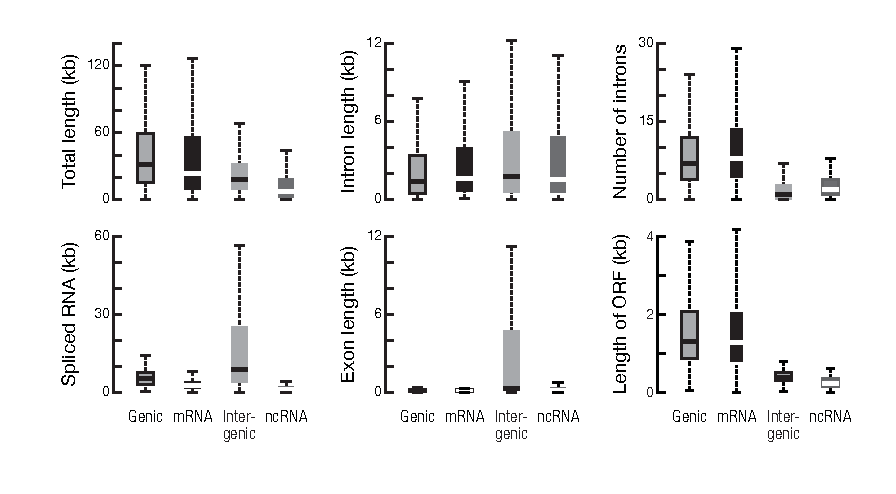
\includegraphics{Figures/SeqZipMethod/piRNAPrecusorTXFeatures.eps}
      \caption[Some general features of piRNA transcripts]
      {
        Some general features of piRNA transcripts\\[0.25cm]
        Top, left) Comparison between genic piRNA precursor transcripts (i.e. pre-pachytene), mRNAs, Intergenic precursor transcripts (i.e. pachytene), and non-coding RNAs (ncRNA) for overall length in nucleotides. Top, middle) Intron length. Top, right) Number of introns. Bottom) Same as above, but considering fully processed (i.e. ``spliced'') versions of the transcripts.
        }
      \label{SeqZipMethod:fig:piRNA precusor Tx features}
      \end{figure}

    An initial goal of characterizing piRNA precursor transcripts was to demonstrate their existence as continuous RNA polymers in total RNA obtained from mouse testes.  Given the tremendous length of these transcripts (Figure \ref{SeqZipMethod:fig:piRNA precusor Tx features}), the go-to experimental approach one would use to demonstrate continuity would be gene-specific RT-PCR. A DNA oligo was designed to hybridize near the 3\textprime~end of the loci \textit{17-qA3.3-27363.1} (\textit{aka} ``M1''), the longest and most studied of the mice piRNA-generating loci. RT would be primed using this oligo, generating cDNAs that would extend (1) until the 5\textprime~end of the transcript was reached or (2) RT fell off the template. Following cDNA generation, pairs of DNA primers hybridizing to 5\textprime~sections of the proposed transcript were used in PCR reactions. Boundaries of the proposed transcript were determined using a combination of small RNA sequencing and poly(A)+-unstranded RNA-Seq. A schematic of the approach is shown in Figure \ref{SeqZipMethod:fig:RT doesn't work for precursors}A.

    One expected issue when performing RT on such a long transcript expressed at low levels is the \textit{lack} of dependence on the RT primer. This is illustrated in Figure \ref{SeqZipMethod:fig:RT doesn't work for precursors}B, where in the ``+RT; -Primer'' lanes there is still a clear signal for all 7 primer pairs. The signal is virtually gone when leaving out RT, suggesting that an RNA template is the source of the signal. It is believed that extremely short DNA species (as short as 4 nt) are priming the RT at some very low rate in the ``-Primer'' reactions. This complication removes RT-PCR as a suitable experimental approach to demonstrate the continuity of piRNA precursor transcripts.

    \begin{figure} % RT doesn't work for piRNA precursor Transcripts
      \centering 
      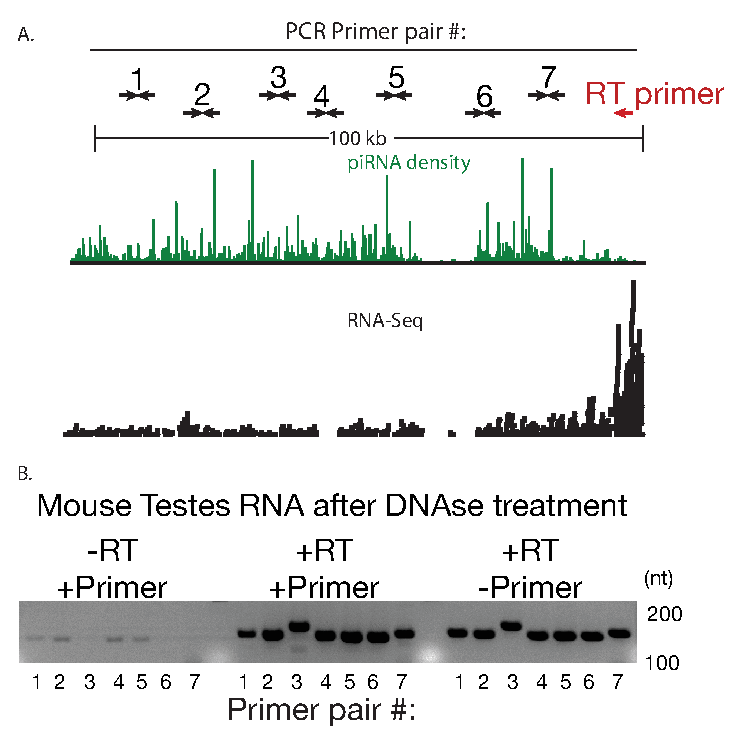
\includegraphics{Figures/SeqZipMethod/RTDoesntWork.eps}
      \caption[pRT Doesn't Work for piRNA precursors]
      {
        RT Doesn't Work for piRNA precursors\\[0.25cm]
        A) Experimental design of RT-PCR demonstration of piRNA precursor \textit{17-qA3.3-27363.1} continuity. Shown in black, numbered 1-7 are primer pairs amplified by PCR, after cDNA generation using the red ``RT primer''. Also shown is the length of the locus, the small RNA signal in green, and the RNA-Seq signal in black. The locus is shown 5\textprime~(left) to 3\textprime~(right). B) Results from RT-PCR using the 7 primer pairs shown in A, and various combinations of $\pm$ RT-primer and RT-PCR enzyme.
      	}
      \label{SeqZipMethod:fig:RT doesn't work for precursors}
    	\end{figure}

  \subsection{Connectivity of Distance Intramolecular Sequences}
    \label{SeqZipMethod:subsec:SeqZip on long RNAs at multiple locations}

    Before applying SeqZip to these extremely difficult transcripts, we designed a set of oligos to demonstrate the continuity of a traditional mRNA. The mRNA picked, \dst{}, was (1) of sufficient length (>23 kb as a fully processed mRNA) and (2) expressed in mouse testes. Ligamers were designed to loop out \textasciitilde5kb sections spaced evenly along the length of the transcript. A ligamer was designed to loop out 22 kb of the message, from 5\textprime~to 3\textprime~end. An illustration of the experimental design is shown in Figure \ref{SeqZipMethod:fig:SeqZip on dst1}.

    \begin{figure} % SeqZip does work for Dst1 transcripts
      \centering 
      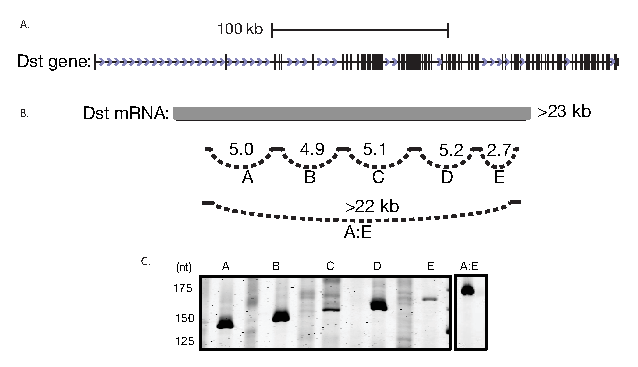
\includegraphics{Figures/SeqZipMethod/dst1.eps}
      \caption[SeqZip on a very long mRNA (\dst{})]
      {
        SeqZip on a very long mRNA (\dst{})\\[0.25cm]
        A) A model of the \dst{} gene. Arrows show direction of transcription (5\textprime~to 3\textprime~). Exons are tall lines, intronic regions join the exons. A scale bar is shown for size in kb. B) A schematic showing how SeqZip was used to investigate 5 different regions of \dst{} transcripts (called A-E). Indicated are the nt of each loop in kb. C) End-point PCR of SeqZip ligation products from each of the ligamer sets shown in (B).
        }
      \label{SeqZipMethod:fig:SeqZip on dst1}
      \end{figure}

    As seen in Figure \ref{SeqZipMethod:fig:SeqZip on dst1}C, ligation products were obtained from every ligamer combination, including the critical set (``AE'') where >22 kb of the message was looped out. In the control experiment, no ligation products were observed. This experiment represents the longest successful ``looping'' in a SeqZip experiment targeting an endogenously expressed RNA.

    An additional demonstration of SeqZip's application to profile long RNAs at multiple sites are experiments involving \fn{}. As described previously (see section \ref{SeqZipPaper:subsec: Method Development and Validation}) \fn{} contains three main sites of alternative splicing: EDB, EDA, and the V-region. Using the proper mix of ligamers, SeqZip examines and maintains connectivity at all three of these sites, correctly reporting on their usage in the RNA template (Figure \ref{SeqZipMethod:fig:Three Site FN1 by SeqZip}). With these results in hand, we felt confident that SeqZip could be used to analyze piRNA precursor transcripts.

    \begin{figure} % Investigating Three sites of FN1 using SeqZip
            \centering 
            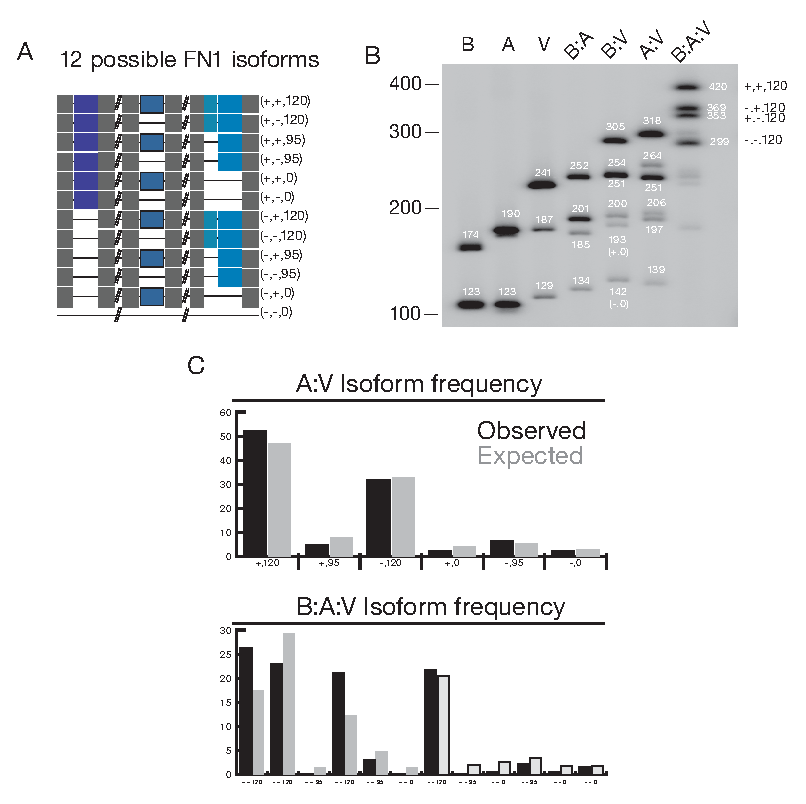
\includegraphics{Figures/SeqZipMethod/fn1ThreeSite.eps}
            \caption[Three sites of alternative splicing in \fn{} by SeqZip]
            {
              Three sites of alternative splicing in \fn{} by SeqZip\\[0.25cm]
              A) Graphical representation of the 12 possible isoforms from mouse \fn{}. B) Radioactive PCR gel showing amplified ligation products templated with specific loops of ligamers. Pools are specified by top row: B = EDB exon only; A = EDA exon only; V = V-Region only; B:A = EDB and EDA exon combinations; B:V = EDB and V-Region combinations; A:V = EDA and V-Region combinations; B:A:V = All two combinations, as shown in panel (A). Marked in nt is shown on left, expected size of specific ligation ligation products indicated in white letters on the gel, or black on right side. Where identity is not obvious from size, identity of isoform provided. C) Quantification of bands from panel (B). Black bars = observed signal of indicated band, Grey = product of individual frequencies. Top only describes A:V combinations, lower shows all combinations.
              }
            \label{SeqZipMethod:fig:Three Site FN1 by SeqZip}
            \end{figure}

  \subsection{Precursor Transcript Continuity}
    \label{SeqZipMethod:sec:piRNA precursor by SeqZip}

    Applying the same logic as that used to examine multiple distant sequences in \dst{} and \fn{}, ligamers were designed against a highly-expressed piRNA-producing loci, \textit{7-qD2-11976} (aka - ``M11''). Five unique sites were picked, again named A-E. Sites were picked to (1) avoid repetitive regions; (2) overlap with expression evidence from small RNA and RNA-Seq data; (3) contain loops of \textasciitilde5 kb in length; and 4) be unique in the genome. A schematic of the approach is shown in Figure \ref{SeqZipMethod:fig:Precursors are testes-specific}A.

    Using total RNA obtained from adult mouse testes, analyzed by SeqZip and the ligamers shown in Figure \ref{SeqZipMethod:fig:Precursors are testes-specific}A, signal from ligation products could routinely be observed from loops of \textasciitilde5 kb (Figure \ref{SeqZipMethod:fig:Precursors are testes-specific}B-left and Figure \ref{SeqZipMethod:fig:M1 analysis by SeqZip}B). Also the signal is dependent on source RNA (Figure \ref{SeqZipMethod:fig:Precursors are testes-specific}B-right) and RNA from mouse spleen did not produce ligation products. The M1 and M11 clusters are both long and have reasonably high expression compared to the other precursors. Yet, no ligation products were ever obtained for either cluster when loops >\textasciitilde5 kb were used (data not shown). What was the cause of this negative signal?

    \begin{figure} % Precursors Transcripts are Testes Specific
        \centering 
        \includegraphics{Figures/SeqZipMethod/testesSpecificRnaseqPrecursors.eps}
        \caption[Testes-specific ligation product signal from piRNA precursor]
        {
          Testes-specific ligation product signal from piRNA precursor\\[0.25cm]
          A) Schematic of the piRNA-producing loci (``gene'') \textit{7-qD2-11976} (aka ``M11'') shown with scale bar, and relative looping ligamer locations.  Loops are labeled A-E, and the length of the loop in kb is shown.  Also shown in green is small RNA expression along this locus. B Left) Ligation products obtained from each set shown in (A) using mouse testes RNA, or B Right) mouse spleen RNA.
        	}
        \label{SeqZipMethod:fig:Precursors are testes-specific}
      	\end{figure}

    \begin{figure} % M1 precusor analysis by SeqZip
        \centering 
        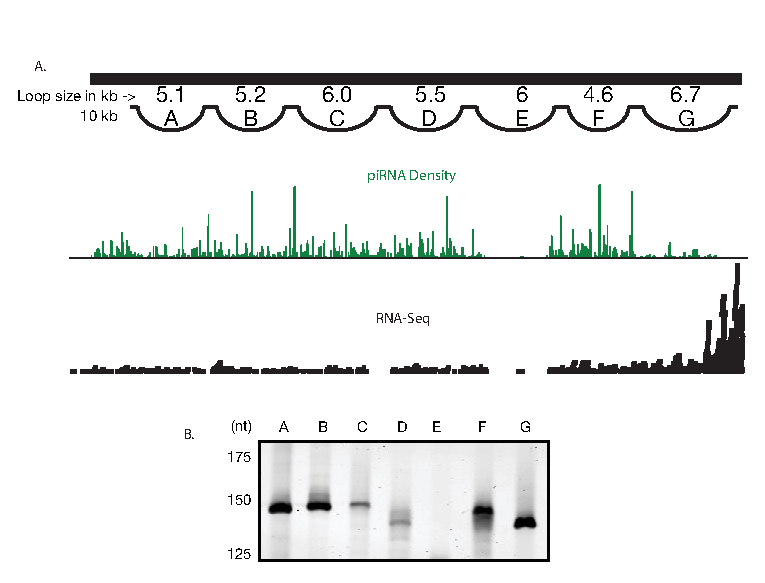
\includegraphics{Figures/SeqZipMethod/piRNAPrecurserAnalyisBySeqZip.eps}
        \caption[SeqZip signal from piRNA-producing loci \textit{17-qA3.3-27363.1}]
        {
          SeqZip signal from piRNA-producing loci \textit{17-qA3.3-27363.1}\\[0.25cm]
          A) Schematic of the piRNA-producing loci \textit{17-qA3.3-27363.1} (aka ``M1'') shown with scale bar, and relative looping ligamer locations.  Loops are labeled A--G and the length of the loop in kb.  Green is small RNA expression along this locus and RNA-Seq in black. B) Ligation products obtained from each set shown in (A) using mouse testes RNA.
        	}
        \label{SeqZipMethod:fig:M1 analysis by SeqZip}
      	\end{figure}

    As first alluded to in Chapter \ref{SeqZipPaper} and discussed in section \ref{SeqZipMethod:sec:Multiplex Gene Study}, ligation efficiency should decrease with loop length and additional required ligations. All of the ligation products used to profile precursors only required two ligation events. Numerous other genes had been investigated with SeqZip that contained >2 sites of ligation (sections \ref{SeqZipPaper:sec:Discussion} and \ref{SeqZipMethod:subsec:SeqZip on long RNAs at multiple locations}). This suggested that the length of the loops was the limiting factor in obtaining ligation products templated off piRNA precursors.

    We investigated this potential explanation by designing a series of ligamer sets with increasing 1 kb increment loop lengths from 5--10 kb. Figure \ref{SeqZipMethod:fig:piRNA precusors and loop length} shows results typical of this series of experiments. The amount of ligation product when using ligamers of increasing loop size decreases with the length of the loop. The signal, after 35 cycles of end-point PCR, is barely visible when the loop is 9 kb, and extremely faint when 10 kb. Ten kilo-bases represents just a fraction of the length of some pachytene piRNA precursor transcripts. 

    \begin{figure} % SeqZip precusor signal decreases with loop length
      \centering
      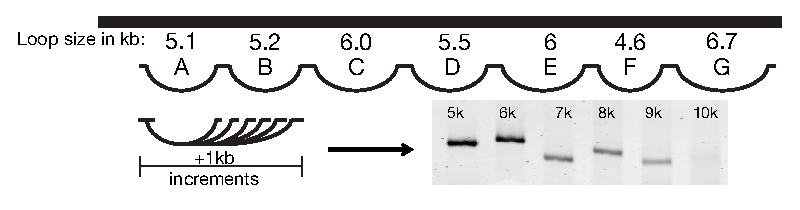
\includegraphics{Figures/SeqZipMethod/piRNAprecusorM1SignalDecreasesWithLoopLength.eps}
      \caption[SeqZip signal from piRNA precursor transcripts decreases with loop length]
      {
        SeqZip signal from piRNA precursor transcripts decreases with loop length\\[0.25cm]
        A series of ligamers were design against the 5\textprime~portion of cluster \textit{17-qA3.3-27363.1} (``M1''). Sets forcing increasing lengths were used, and ligation products were analyzed by end-point PCR.
        }
      \label{SeqZipMethod:fig:piRNA precusors and loop length}
      \end{figure}

    Even after numerous attempts, ligation products could not be obtained for loop sizes >10 kb, no matter what the target transcript. At this point in the study, we decided to abandon the demonstration of piRNA precursor transcripts as continuous transcripts via SeqZip, and instead turned our attention to splicing within the transcripts (discussed in the next section, \ref{SeqZipMethod:sec:piRNA precursors are spliced}) which eventually lead to the study presented in Chapter \ref{MolCel}.

    What could be the cause of our inability to create ligation products? The method worked so well, without any optimization, for mRNAs of similar length and expression (e.g. \dst{}). Our current hypothesis is that at steady-state levels, the amount of full-length piRNA precursors that exist---in continuous polymers of length >10kb---is extremely low. Low to the point of being below the SeqZip limit of detection. Indeed, many nucleases appear to act on piRNA precursors along their journey from Pol II transcript to mature piRNA (see section \ref{Intro:subsec:Processing of piRNAs in mice}). The piRNA machinery is perhaps too fast and efficient for us to capture these extremely long RNAs. Future experiments that somehow perturb the pathway, such as \textit{Pld6} (aka \textit{MmZuc, MitoPLD} and \textit{Zucchini} in flies) could accumulate precursors before cleavage occurs.

\section{Precursor Splicing}
  \label{SeqZipMethod:sec:piRNA precursors are spliced}

  Once it was determined that the existence of piRNA precursor transcripts as continuous piRNA precursors could not be demonstrated using SeqZip, careful attention was paid to RNA-Seq data used to determine the edges of precursor loci transcription. The RNA-Seq data, once aligned with a splicing-sensitive algorithm (i.e. ``Tophat'' \citep{Trapnell2009}), showed that piRNA precursors were spliced. Multiple reads and species supported intronic segments and each contained little to no RNA-Seq and small RNA reads. A good example of the high-level type of data observation that was being performed until this point is shown in Figure \ref{SeqZipMethod:fig:evidence for precusor splicing}. In this figure, small RNA data is shown in green along with RNA-Seq data in black. For this particular cluster, the RNA-Seq data and small RNA data appear continuous with the length of gene, as typical for many loci in \flies{}. It was necessary to increase the resolution used to study the piRNA-generating loci in mice in order to accurately define transcripts.

  \begin{figure} % evidence for precursor splicing
    \centering 
    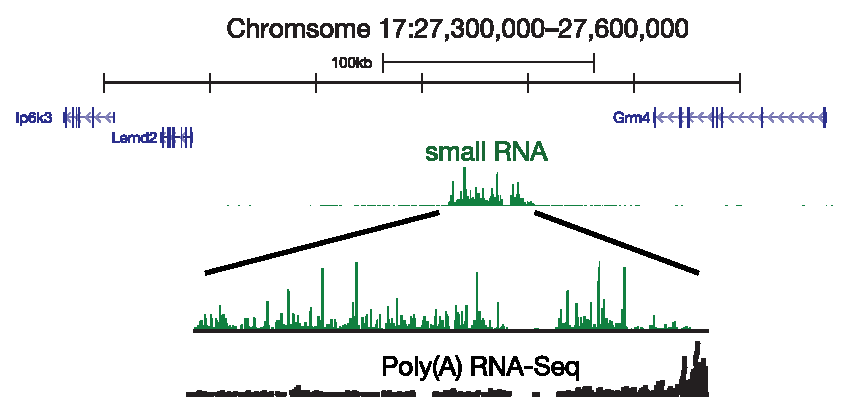
\includegraphics{Figures/SeqZipMethod/evidenceForPrecursorSplicing.eps}
    \caption[Example small RNA and RNA-Seq data aligned to a piRNA-generating loci]
    {
      Example small RNA and RNA-Seq data aligned to a piRNA-generating loci (\textit{17-qA3.3-26735})\\[0.25cm]
      Show in the context of the genome and surrounding genes (blue) is a piRNA-generating loci, with signal in green. Bottom) zoomed view of the small RNA signal (green) along with poly(A)+-unstranded RNA-Seq (black).
      }
    \label{SeqZipMethod:fig:evidence for precusor splicing}
    \end{figure}

  One of the most illustrative piRNA-generating loci is that containing the genes \textit{17-qA3.3-27363.1 and 17-qA3.3-26735} (Figure \ref{SeqZipMethod:fig:no piRNAs within Precursor Introns}). These two genes are expressed in pre-pachytene testes and increase expression once mice hit 14.5 dpp. These two genes along account for 27\% of all the piRNAs sequenced at 14.5 dpp (see Chapter \ref{MolCel} and Table \ref{SeqZipMethod:tab:matchedClusterValues}). A extremely informative feature, detected early from initial poly(A)+-unstranded RNA-Seq libraries, was the absence of signal near the apparent 3\textprime~end of the loci. There were many reads that could be aligned across this gap, as if it was a traditional mRNA intron. There were no repeat element that would have depleted this region of the message for reads, as with other sections of the locus. The most obvious explanation was that the precursor contained an intron, which was spliced out prior to poly(A) tailing..

  \begin{figure} % No piRNAs in introns
    \centering 
    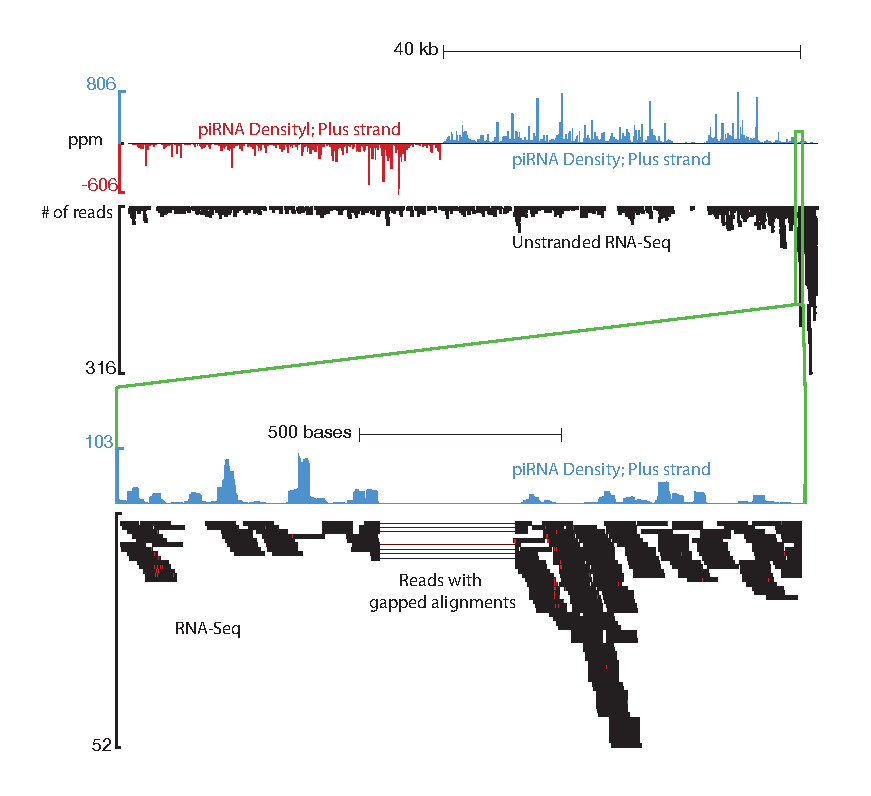
\includegraphics{Figures/SeqZipMethod/noPiRNAswithinPrecusorIntrons.eps}
    \caption[Introns in mammalian piRNA precursors]
    {
      Introns in mammalian piRNA precursors\\[0.25cm]
      Top) Divergently transcribed piRNA-producing genes \textit{17-qA3.3-27363.1 and 17-qA3.3-26735}. These genes are transcribed from a common promoter. Plus strand small RNAs are shown in blue, minus stranded small RNAs in red. poly(A)+-unstranded) RNA-Seq is shown in black. Bottom) Zoomed portion of the message near the 3\textprime~end of \textit{17-qA3.3-26735}. Plus-stranded small RNA (blue) and RNA-Seq reads in black. Multiple RNA reads and species aligned across a intron. This region was also largely free of small RNA signal.
      }
    \label{SeqZipMethod:fig:no piRNAs within Precursor Introns}
    \end{figure}

  The results shown in Figure \ref{SeqZipMethod:fig:no piRNAs within Precursor Introns} were very exciting initially, and provided important clues to the biogenesis of piRNAs. The presence of an intron indicates Pol II origin. The lack of small RNA within the intron supported mature piRNA creation after precursor splicing. A major reason why this feature had not already been noticed is that small RNA data is not long enough to accurately and confidently align across splice junctions. Therefore, intron detection had to wait for application of longer RNA-Seq reads and splicing-sensitive alignment software. Once these introns were known, supporting their use with small RNA data become possible.

  Using genomic coordinates supplied by the splicing-sensitive alignment algorithm \citep{Trapnell2009}, an alignment index of transcript sequences \textit{flanking} the introns was created. Then, using a more traditional (in terms of small RNA alignment) aligner, Bowtie \citep{Langmead2009}, those piRNAs that did \textit{not} map to the genome could be aligned to index containg piRNA precursor splice junctions. This experiment is shown graphically in Figure \ref{SeqZipMethod:fig: piRNAs map to SJ}.

  \begin{figure} % piRNAs map to splice junctions
    \centering 
    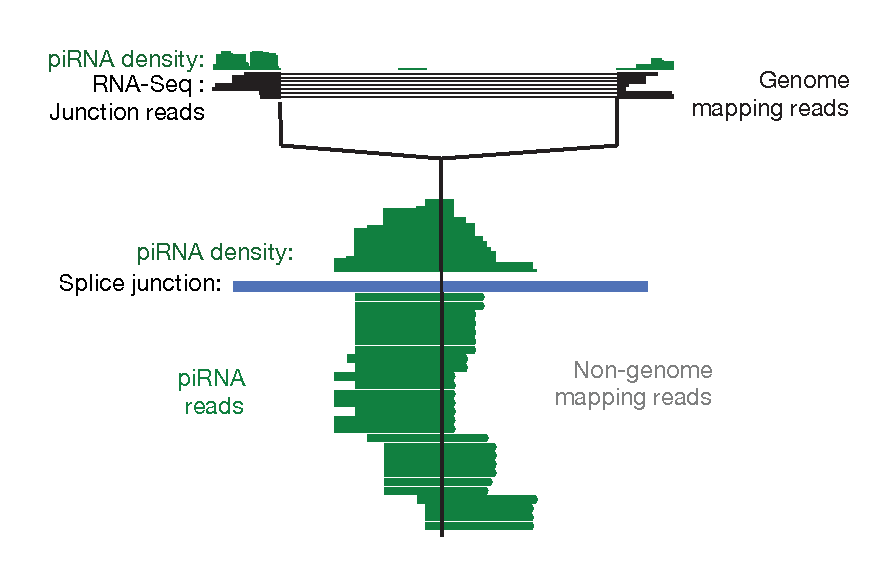
\includegraphics{Figures/SeqZipMethod/smallRNAsMapToPrecursorSJ.eps}
    \caption[piRNAs map to precursor transcript splice junctions]
    {
      piRNAs map to precursor transcript splice junctions\\[0.25cm]
      Top) piRNA density (green) and RNA-Seq density at the 3\textprime~most intron within \textit{17-qA3.3-26735}. Bottom) A splice junction sequence (blue) created by joining the sequences just outside the intron shown in (Top) is sufficient to align non-genome mapping piRNAs.
      }
    \label{SeqZipMethod:fig: piRNAs map to SJ}
    \end{figure}

  Chapter \ref{MolCel} discusses the ultimate refinement of the observations described above, including the generality of splicing within precursor transcripts. In fact, there are a total of 383 introns within the ``intergenic'' sub-classified 214 piRNA-generating loci from \citep{Li2013e} (see Table \ref{Appendix:tab:GenicAndInterGenicLoci}). These introns display a A-MYB\textendash dependent small RNA signal across their exon-exon junctions (Figure \ref{SeqZipMethod:fig: amyb makes SJ mapping}). The more traditionally looking piRNA-producing loci of the ``genic'' subclass, contain far more introns (2,113). The signal for these transcripts does not display the same A-MYB\textendash dependent small RNA signal.

  \begin{figure} % A-Myb mutants do not have SJ-mapping piRNAs
    \centering 
    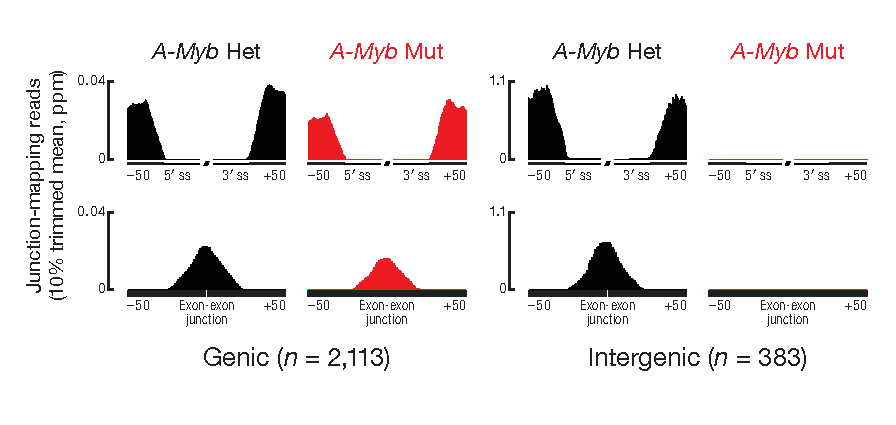
\includegraphics{Figures/SeqZipMethod/aggregatePiRNAsatSpliceJunctions.eps}
    \caption[\amyb{} Mutants produce no splice-junction mapping piRNAs for genic piRNA-producing loci]
    {
      \amyb{} Mutants produce no splice-junction mapping piRNAs for genic piRNA-producing loci\\[0.25cm]
      Trimmed mean ppm of junction-mapping piRNAs within two classes (``genic \& Intergenic'') loci. Shown in red is signal from \amyb{} mutant mice, black \amyb{} heterozygous mice. All data from stranded RNA-Seq (strand accounted for during alignment and signal aggregation).
      }
    \label{SeqZipMethod:fig: amyb makes SJ mapping}
    \end{figure}

  While it was not possible to demonstrate continuity of piRNA-producing precursors using SeqZip, development of advanced HTS methods and computational approaches provides clear evidence that they are (see Chapter \ref{MolCel}). Proposed future experiments into mammalian piRNA precursors are discussed in section \ref{Disc:sec:piRNA precursors}.

\cleardoublepage